\begin{artengenv}{Paweł Kawalec}
	{The process of microRNAs discovery}
	{The process of microRNAs discovery}
	{The process of microRNAs discovery}
	{John Paul II Catholic University of Lublin}
	{The widespread particularist account of the onset of molecular biology that identifies it with the discovery of the DNA structure in 1953 has been recently contested. The paper contributes to this debate by focusing on a more recent discovery of small noncoding RNAs (microRNAs). First, it outlines a particularist account of the microRNAs discovery and the origins of the particularist predilection of the modern scientometric studies of science dynamics. Next, it discusses its limitations and proposes an alternative, modified processualist account of the discovery. In the final part, the paper applies this approach to unravel network dynamics of the research on the first two microRNAs that were discovered, namely \textit{lin}-4 and \textit{let}-7.
	}
	{breakthrough research, let-7, lin-4, particularism, processualism, scientific discovery, research routine, microRNAs, noncoding RNA.}


\section{Introduction}
\lettrine[loversize=0.13,lines=2,lraise=-0.01,nindent=0em,findent=0.2pt]%
{W}{}ith the demise of WWII the dynamics of science has become an object of intense interest in economics, scientometrics, sociology, and, last but not least, in studies on history and philosophy of science. A view that predominated those discussions mostly concerned isolated outcomes of scientific research, such as new theories, models, as well as experimental and observational data. Of course, the focus was on the most widely publicized ones, such as the double helix structure of DNA. Here, I will refer to this view as particularism
%\label{ref:RNDX87ygmnHU2}(Kawalec, 2020).
\parencite[][]{giovagnoli_cognitive_2020}. %
 The opposite view, namely processualism, perceives scientific change as a continuous process of conceptual evolution inherent in research activities that generate new concepts, new relationships between the existing ones or their applications in new fields that, in turn, trigger new research processes 
%\label{ref:RNDgMRbwnXrYt}(Nicholson and Dupré, 2018).
\parencite[][]{nicholson_everything_2018}. %
 The examination of microRNAs in this paper substantiates a modified version of processualism that combines the inherent dynamics of continuous change with external shocks, such as institutional or technological developments.

The paper proceeds as follows. First, I outline a purported particularist account of microRNAs discovery and then I present the origin of the particularist predilection of scientometric measures of science dynamics. Next, I indicate limitations of particularism and, as alternative, propose a modified processualist account of the discovery. In the final part, I apply this approach to examine network dynamics of the research subroutines concerning the first two microRNAs that were discovered, namely \textit{lin}-4 and \textit{let}-7.

\section{Particularist account of the microRNAs discovery}
In 1993 two research teams led by Victor Ambros and Gary Ruvkun, respectively, published papers reporting a new kind of RNA particle: \textit{lin-4}. The well-known central dogma identified the main---and presumably exclusive---role of RNA as the template for protein sequences.\footnote{There is some discrepancy between the original formulation of the central dogma by F. Crick
%\label{ref:RNDTAwGDm5AsM}(1958, 1970)
\parencite*[][]{crick_central_1970} %
 and its ``lucid presentation'' 
%\label{ref:RNDUB41shCuDU}(Watson, 1965, pp.297–298)
\parencite[][pp.297–298]{watson_molecular_1965} %
 by S.~Spiegelman and M.~Hayashi 
%\label{ref:RNDVMNFyp8qd8}(1963).
\parencite*[][]{spiegelman_present_1963}. %
 While Crick's version, essentially, only precludes the information transfer from proteins to DNA or RNA, Spiegelman and Hayashi require one-directional information transfer from RNA to protein, excluding thereby two other routes that are possible in Crick's version. I am grateful to one of the Reviewers for pointing that out.} However, the RNA discovered in 1993 had a different function: it regulated gene expression without encoding any protein. What the two teams demonstrated was that in nematode \textit{Caenorhabditis elegans} (\textit{C. elegans} in short) the gene \textit{lin-4} negatively regulates translation of another gene \textit{lin-14} that, in turn, codes LIN-14 protein. When this mechanism is corrupted by a mutation of \textit{lin-4} causing its loss-of-function, \textit{C. elegans} reiterates early fates at late developmental stages, being unable to develop adult structures and to lay eggs 
%\label{ref:RNDl5HcelhTv8}(Lee, Feinbaum and Ambros, 1993).
\parencite[][]{lee_c_1993}. %
 The authors succinctly summarize two lines of evidence supporting the claim that \textit{lin-4} does not encode protein:

\begin{quotation}
First, strategically located frameshift and nonsense mutations, as well as an ATG to ACG mutation, were introduced into several putative open reading frames of the \textit{C. elegans} genomic clone without affecting rescuing activity. Second, comparison of the \textit{C. elegans}, \textit{C. briggsae}, \textit{C. remanei}, and \textit{C. vulgaris} \textit{lin-4} genomic sequences (which are functionally interchangeable in \textit{C. elegans}) revealed a high level of nucleic acid sequence conservation but no conserved open reading frames. Regions of conserved sequence do not show a degeneracy at the third base positions of putative codons that would be expected for protein coding sequences, and they contain deletions or insertions that would cause frameshifts. There are no splice donor or acceptor sites that would compensate for these frameshifts. Thus, if a conserved protein product were encoded by the \textit{lin}-4 locus, its synthesis would need to be directed by unorthodox translation start and stop signals. The 893 bp \textit{C. elegans} fragment rescues in either orientation, arguing against the generation of a \textit{lin-4} protein from the rescuing fragment using translational signals from the vector
%\label{ref:RNDyLktpnv548}(Lee, Feinbaum and Ambros, 1993, p.849).
\parencite[][p.849]{lee_c_1993}.%


\end{quotation}
Further evidence was brought about by providing the molecular mechanism of antisense complementarity of the \textit{lin-4} transcripts to the \textit{lin-14} 3'UTR
%\label{ref:RNDJSCLPJle8g}(Wightman, Ha and Ruvkun, 1993).
\parencite[][]{wightman_posttranscriptional_1993}. %
 As it turns out, this complementarity is conserved between \textit{C. elegans} and \textit{C. briggsae}. Moreover, the loss-of-function mutation of \textit{lin-4} is located within the block of those complementary sequences, indicating a more universal character of this mechanism. As Ambros and his collaborators emphasized: ``These observations strongly support the hypothesis that \textit{lin}-4 downregulates LIN-14 protein levels through a direct RNA–RNA interaction with the \textit{lin}-14 3'UTR''
%\label{ref:RNDtP5yc622Rk}(Lee, Feinbaum and Ambros, 1993, p.850).
\parencite[][p.850]{lee_c_1993}.%


As \textit{lin-4} was thought to be a worm-specific phenomenon, this discovery remained almost unnoticed until Ruvkun's laboratory came up with another discovery. They demonstrated that while \textit{let-7} is another non-coding RNA
%\label{ref:RNDygVcPnBHyy}(Reinhart et al., 2000),
\parencite[][]{reinhart_21-nucleotide_2000}, %
 it is demonstrably present in ``a wide range of animal species, including vertebrate, ascidian, hemichordate, mollusc, annelid and arthropod'', including humans, and is highly evolutionarily conserved 
%\label{ref:RNDhIQ8V8gVOW}(Pasquinelli et al., 2000, p.86).
\parencite[][p.86]{pasquinelli_conservation_2000}.%


Soon, other research teams joined in and this resulted in identification of new kinds of non-coding RNAs, which---with the publication of the issue 294(5543) of \textit{Science} in 2001---started to be called ``microRNAs'' (or, alternatively, ``miRNAs''). The relevance of microRNAs to oncogenesis was soon recognized
%\label{ref:RNDbhW0AHfZYg}(Calin et al., 2002)
\parencite[][]{calin_frequent_2002} %
 and epitomized by a new category ``oncoMIRs'' 
%\label{ref:RND465rHz6bTI}(He et al., 2019).
\parencite[][]{he_oncomir_2019}.%
\footnote{A particularist scientometric measure misidentified the onset of microRNAs research by 13 years and attributed it to a review paper, for a detailed exposition see 
%\label{ref:RND2JPtEbdK4r}(Kawalec, 2020).
\parencite[][]{giovagnoli_cognitive_2020}.%
} This early stage of research 
%\label{ref:RND71CEb42YEz}(Kawalec, 2018)
\parencite[][]{kawalec_transformations_2018} %
 on microRNAs may be summarized by the following sequence:
$$
\textit{lin-4 –– lin-7}\text{ –– microRNAs –– oncoMIRs –– \ldots}
$$

This sequence apparently captures the early milestones in the discovery of microRNAs. Moreover, it seems to reflect the growth regularity identified by Derek J. de Solla Price
%\label{ref:RNDi0FXtnGFoH}(de Solla Price, 1986).
\parencite[de][]{de_solla_price_little_1986}. %
 In studying various research domains he established that the growth is manifested by the natural logistic curve (inverted S-curve), similar to the one presented in figure \ref{fig1kawalec}.

Before my discussion of the sequence of discoveries related to microRNAs and the corresponding de Solla Price's growth curve, let me examine the origins and presumptions of the particularist approach to the advancement of science.
\begin{figure}[h!]
	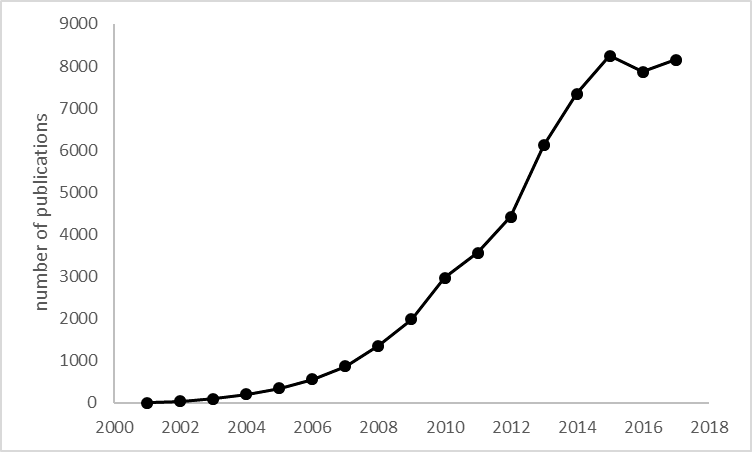
\includegraphics[width=1\textwidth]{ART_Kawalec/Kawalec-img001bw.png}
%	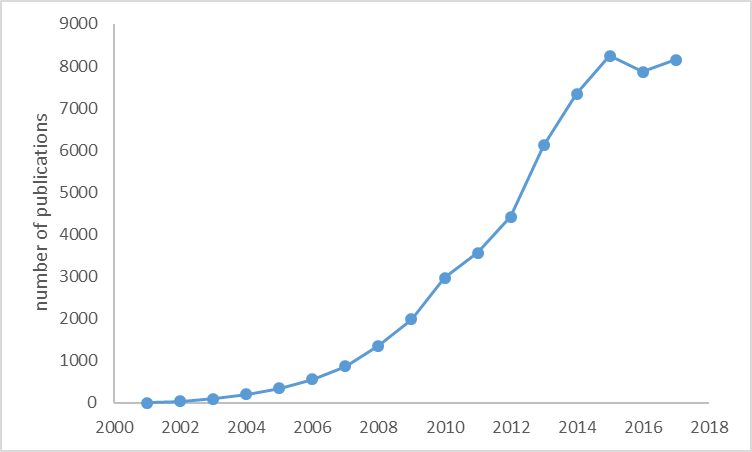
\includegraphics[width=1\textwidth]{ART_Kawalec/Kawalec-img001.png}
	\caption{The annual growth of publication number on microRNAs. Source: own analysis of MEDLINE dataset for ``microRNAs'' as MeSH keyword.}\label{fig1kawalec}
\end{figure}



\section{Particularist predilection of scientometric measures of science dynamics}
Despite divergence between the initial de Solla Price's micro (logistic curve) and Kuhn's macro (theory of paradigms) perspectives on science dynamics
%\label{ref:RNDSPq9qFoV4e}(Shapin, 2015)
\parencite[][]{shapin_kuhns_2015} %
 they merged adopting the latter's particularist view. Kuhn in his 1969 \textit{Postscript} to \textit{The Structure of Scientific Revolutions}, originally published in 1962, defines ``paradigm'' by reference to scientific community: ``A paradigm is what the members of a scientific community share'' 
%\label{ref:RNDmOpL7aSSlG}(Kuhn, 1970, p.176).
\parencite[][p.176]{kuhn_structure_1970}. %
 One way to avoid vicious circularity in this characterization that Kuhn considers is by providing an independent identification of scientific communities, a task he would gladly relegate to sociologists and historians of science. In referring to ``preliminary results'' on this path he explicitly refers to publications concerning citation patterns of Derek~J. de Solla Price and Eugene Garfield, the two founding fathers of scientometrics 
%\label{ref:RNDQu3nw8129W}(Kuhn, 1970, p.178 n.6).
\parencite[][p.178 n.6]{kuhn_structure_1970}. %
 Kuhn's ``naturalistic'' approach to science was subsequently ``enthusiastically incorporated'' into social-constructivist work \textit{via} the ``strong programme'' of Barry Barnes and David Bloor 
%\label{ref:RNDj43g7EUSjc}(Shapin, 2015).
\parencite[][]{shapin_kuhns_2015}. %
 Steve Fuller 
%\label{ref:RNDsh9a8sO9xR}(Fuller, 1992, p.270 n.107)
\parencite[][p.270 n.107]{fuller_being_1992} %
 notes a more direct connection between Kuhn and Price: ``the Kuhnian life cycle [of old paradigm-anomalies-crisis-revolution-new paradigm] is ‘Price's Index,' which measures the obsolescence rate of journal articles in terms of diminishing citation patterns. A rapid obsolescence rate means a rapidly advancing research front, a paradigm at top puzzle-solving performance levels\footnote{For a more detailed exposition of ``Price's index'', see 
 %\label{ref:RNDvugEcFboHB}(De Mey, 1982, pp.148–170).
 \parencite[][pp.148–170]{de_mey_cognitive_1982}.%
 }.''

Fuller, commenting on the affinity between Kuhn's and Price's theories of science dynamics, observes that it strongly affected how scientometricians designed ``quantitative measures for tracking the growth of knowledge'' in view of ``science policy concerns''. This approach is marked by characteristically particularist focus: ``[...] the major ‘product' of science is presumed to be the journal article, whose value is measured in terms of the other articles that cite it as instrumental in their own production. What makes today's science so ‘big,' then, is the number of articles produced, and especially the exponential rate at which they are being produced. [...] Price seems to be impressed with the fact that out of a myriad of national interests can emerge a global picture of science that is reducible to fairly simple and intuitive logistic curves [...]''
%\label{ref:RND7zMstr1jqu}(Fuller, 1992, pp.270–271).
\parencite[][pp.270–271]{fuller_being_1992}. %
 The overall dynamics of science, thus, results from aggregating individual publications and their co-citation patterns. It, therefore, explains why the particularist predilection has become a predominant view in various approaches in theory of science. In the following section I argue that this kind of particularistic approach is too simplistic and the overall dynamics results from an interaction of different kinds of processes 
%\label{ref:RNDYsXpqqPa9M}(Kawalec, 2020),
\parencite[][]{giovagnoli_cognitive_2020}, %
 the understanding of which preconditions our grasp of the dynamics of science.

\section{Processualist account of microRNAs discovery }
Particularist accounts of scientific progress face a number of challenges
%\label{ref:RNDbiB7GpylJ2}(Losee, 2004).
\parencite[][]{losee_theories_2004}. %
 Let me focus on two general ones, pertaining to the case of microRNAs. The first general problem, referred to here as \textit{the} \textit{granularity problem}, is concerned with the appropriate identification of the game-changer. The possibilities range here from a single publication, such as Copernicus's \textit{De Revolutionibus} or Newton's \textit{Principia}, to an extended period covering 300 years, as argued by Rupert Hall in his monumental \textit{The Scientific Revolution: 1500–1800} 
%\label{ref:RNDgseuFzcmxg}(Hall, 1954).
\parencite[][]{hall_scientific_1954}. %
 Hall's idea is that while prior to 1500 there was no scientific research characteristic of modern science, combining experimentation with mathematical language, it had been definitely established by the beginning of the 19\textsuperscript{th} century. Perhaps, none of the individual contributions, such as Copernicus's or Newton's, were sufficient to establish the practice of modern science as understood by Hall. However, the rounded dates disguise the apparent continuity with both, the prior and subsequent research. On the other hand, the individual publications are not comprehensible without reference to previous accomplishments, such as Ptolemy's astronomy or Kepler's laws, respectively. Hence, the task to isolate a particular research process as the moment of revolutionary or breakthrough change, seems rather hopeless.

Nevertheless, even if we suppose that such a precise and unproblematic identification would be possible, it encounters another problem, referred to here as \textit{the reference class problem}. A particular discovery or publication may be perceived as revolutionary from the perspective of quite different points of view, taking into account different antecedent and subsequent accomplishments. One example is Lavoisier's chemical revolution
%\label{ref:RND86PBbivVjI}(Losee, 2004, p.66).
\parencite[][p.66]{losee_theories_2004}. %
 On one reading it constituted the culmination of a ``Stahlian revolution'' which ``emancipated chemistry from the domination of physics''. Hence, against this background, it would be best understood in opposition to the Newtonian theory which claimed that matter comprises homogeneous particles by demonstrating the existence of qualitatively distinct chemical elements. Alternatively, Lavoisier's work is seen as a preliminary stage culminating in the subsequent works of Dalton who was able to assign relative atomic weights to elementary species. Thus, a change of the reference class would result in a corresponding change in the particularist identification of the bearer of scientific revolution.

These problems indicate a need for an alternative account of scientific progress. So, let us now turn to one such alternative, namely the processualist standpoint. This brings us back to section 2, but now I will try to provide the processualist description of the early stages of the development of microRNAs as a new \textit{research routine}. The concept of research routine has been recently proposed as an alternative to traditional perspectives on research dynamics, which isolate its cognitive or social/institutional aspects and are confined to a particular area, such as philosophy, social studies of science or scientometrics. Research routine as a repeated and recognizable pattern of research practices of a scientific community (within Merton's ``invisible college'') sharing a symbolic representation (such as concept, classification, model or theory) integrates cognitive and institutional network dynamics of research processes, as exemplified by the examination of microRNAs research in
%\label{ref:RNDZPMNWLPU8u}(Kawalec, 2018).
\parencite[][]{kawalec_transformations_2018}. %
 In the next section, I identify two kinds of mechanisms underlying the dynamics of the microRNAs research routine.

On the wide-spread view of the history of molecular biology the identification of the structure and function of the double helix of DNA in 1953 set the stage for the subsequent development of molecular biology as a separate discipline. However, this view is not historically adequate as it downplays the role of the antecedent research on proteins and subsequent intense research concerning the role of RNAs that intermediated between DNA and proteins
%\label{ref:RNDBfvnn35yrA}(García-Sancho, 2012).
\parencite[][]{garcia-sancho_biology_2012}.%
\footnote{I am grateful to one of the Reviewers for stressing this point.} As. J. Darnell succinctly puts it: ``The bold discovery by James Watson and Francis Crick of the structure of DNA, often told, and well told, by the protagonists themselves, is frequently recited as the ‘start' of molecular biology. And if one watershed discovery is to be chosen as the ‘beginning,' that discovery is it. But there was a preceding half-century struggle of genetics and physical biochemistry [...]'' 
%\label{ref:RNDe6bPAtwv5V}(Darnell, 2011, p.2).
\parencite[][p.2]{darnell_rna_2011}. %
 The period 1950–1980 that followed recognized ``the centrality of RNA to life'' due to plentiful discoveries of the types of RNA molecules and their specific functions (esp. tRNA, ribosomes, mRNA, pre-mRNA, pre-rRNA, RNA splicing, etc.). This process of gradual realization of the importance of RNA is well epitomized by the \textit{RNA world} hypothesis concerning the initial phase in the evolution of life. The detailed account of research advancements concerning RNA in the period of 1953–1980 by Darnell 
%\label{ref:RNDpzNwn6PmtN}(2011)
\parencite*[][]{darnell_rna_2011} %
 undermines the widespread particularist focus on the discovery of the double helix as the sole ``start'' of molecular biology.

Of course, the discovery of microRNAs as noncoding small RNAs is entrenched in these conceptual advances in RNA investigations that began in 1953. The laboratory practices that made this discovery possible include Syndey Brenner's work on the genetics of \textit{C. elegans} in the late 1960's and early 1970's that established this nematode as the model organism for genetic studies. Robert Horvitz and his collaborators by 1980 identified cell lineages for \textit{C. elegans} and its mutant forms (24 in total), including two ``heterochronic'' genes \textit{lin-4} (short from ``lineage abnormal'') and \textit{let-7} (``lethal''). Further, Horvitz and his post-docs, Ambros and Ruvkun, in the late 1980s were able to identify the functional model specifying interdependence between heterochronic genes in \textit{C. elegans}, focusing on the relation between \textit{lin-4} and \textit{lin-14}. The famous paper
%\label{ref:RNDM85sa5wRCR}(Lee, Feinbaum and Ambros, 1993)
\parencite[][]{lee_c_1993} %
 provided the details of the molecular model of the regulatory mechanism between the two genes. These accomplishments were accompanied by a flow of changes in experimental techniques 
%\label{ref:RNDpIrYhbF31B}(Kawalec, 2020).
\parencite[][]{giovagnoli_cognitive_2020}. %
 Further research on \textit{C. elegans} resulted in the discovery of RNA interference (RNAi) in 1998. Soon thereafter, Ruvkun and his collaborators identified the second microRNA, namely \textit{let-7} and demonstrated its high evolutionary conservation. Several laboratories instantly joined in, including Tom Tuschl's and David Bartel's searching for new microRNAs both in \textit{C. elegans} as well as in other organisms. These early findings were jointly reported in 2001 in \textit{Science} 
%\label{ref:RNDIa8ZxSmJSb}(Lagos-Quintana et al., 2001; Lau et al., 2001; Lee and Ambros, 2001).
\parencites[][]{lagos-quintana_identification_2001}[][]{lau_abundant_2001}[][]{lee_extensive_2001}. %
 A new line of research was initiated by the team led by George Calin who first documented a relation between oncogenesis and deletion or down-regulation of microRNAs as early as 2002. Subsequent research on microRNAs included, for instance, prediction of targets, biogenesis, identification of microRNAs in different organisms, diagnostic and therapeutic potential, occurrence in body fluids and identification of other noncoding RNA particles. It has ``revealed that miRNAs play important roles in diverse processes such as cell differentiation, cell proliferation, and organ development. More importantly, beyond their roles in physiological processes, extensive research has explored miRNA involvement in various pathologies, including infectious diseases'' 
%\label{ref:RNDAMNvOo87Va}(Fu et al., 2011, p.4246).
\parencite[][p.4246]{fu_circulating_2011}. %
 The end of the early phase in development of microRNAs research routine is marked by 2006 when the next-generation sequencing methods enabled more efficient research.\footnote{For a systematic exposition of the phases in microRNAs research, see 
%\label{ref:RNDhrMaHpUTcC}(Kawalec, 2018).
\parencite[][]{kawalec_transformations_2018}. %
 In private communication this account has been approved by Victor Ambros and Robert Horvitz.}

Without going too much into the details, let me give a perspicuous illustration of the processual nature of the discovery of microRNAs. The initial discovery of the molecular regulatory mechanism between \textit{lin-4} and \textit{lin-14} in 1993 was initially perceived as a phenomenon specific to \textit{C. elegans} and, perhaps, related nematodes. It was only the subsequent discoveries of the universal RNAi mechanism in 1998 and the second microRNA \textit{let-7} with its high evolutionary conservation in 2000 that eventually established a new taxonomic category of ``microRNAs'' in 2001. So, the two publications that appeared in 1993 only with this hindsight can be retrospectively recognized ``a breakthrough''. The pressing question to proponents of particularism would now be: When the discovery of microRNAs actually took place? Was it just 1993,\footnote{Note that the main results were actually known earlier, but intentionally withheld from publication for several months.} or the whole 8-year period?, or, perhaps, an even longer one, if one would like to consider more recently discovered ``oncoMIRs'' or ``circulating microRNAs''?

\section{Varied mechanisms of science dynamics: the fate of \textit{lin-4} and \textit{let-7}}
In the preceding section I indicated the granularity and reference class problems as the reasons why the particularist view of the dynamics of microRNAs, as depicted on Figure \ref{fig1kawalec}, may be misleading. Yet, there is another reason why this may be so. The simplistic pronouncements of particularists may turn our attention away from the complexity of the mechanisms underlying the dynamics. In this section I will provide a detailed illustration of such a complexity as exemplified by two research sub-routines concerning the first two microRNAs discovered, namely \textit{lin-4} and \textit{let-7}.

One way to grasp the overall dynamics of microRNAs routine is to observe how the entire network, such as co-authorship of publications, develops. The tools provided by network analysis allow one to trace how ``the invisible college''
%\label{ref:RNDi5rOEY3AmT}(Merton and Garfield, 1986, pp.viii–ix)
\parencite[][pp.viii–ix]{merton_foreword_1986} %
 develops with a new routine. An important indicator of this dynamics is ``the giant component'' of a given network that forms the largest set within the network of authors who are ``connected'' by their collaboration. In case of an emerging routine the whole network is dispersed and the giant component is hardly distinguishable from other groups of connected papers. In other words, there is no clear indication of a dominance of a particular group of authors. And, to use Merton's wording, it could be interpreted as a stage where no invisible college can be clearly identified.

In contrast, mature routine is characterized by the clearly present, and dominant, giant component. Usually, the critical point is 50\% of all nodes, such as authors, in the given network. Figure \ref{fig2kawalec} contrasts two stages of the development of the author network with links signifying co-authorship relations. The 1993 stage captures the early phase of microRNAs routine development with Horvitz as the leader of the ``giant'' component. However, at this stage, the routine is still in its infancy as the ``giant'' component embraces only 26 people, that is 11\% of all the authors. In 2018 the routine is apparently mature: while the giant component consists of 70\% of all the authors, their total number increased by an astonishing (almost) 100 times.

\begin{figure}[h!]
\begin{flushleft}
\tablefirsthead{}
\tablehead{}
\tabletail{}
\tablelasttail{}
\begin{tabular}{m{.5\linewidth}|m{.5\linewidth}}
{\centering\bfseries 1993\par}

 &
{\centering\bfseries 2018\par}

\\
 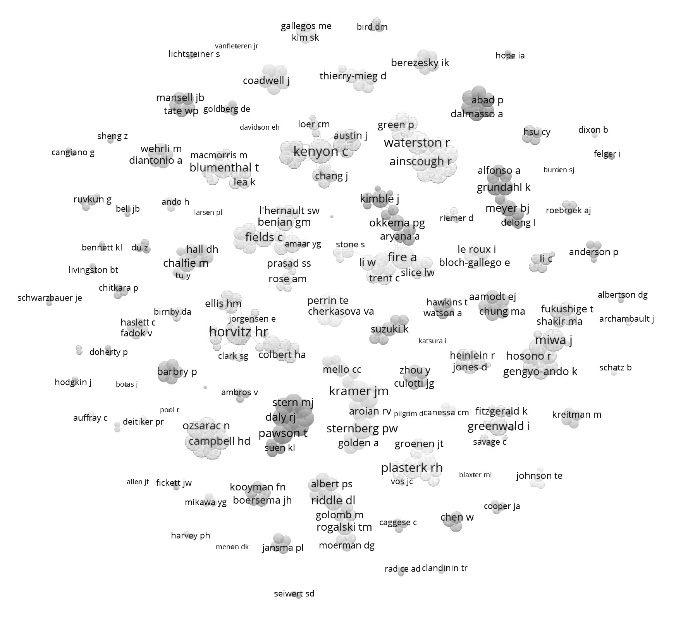
\includegraphics[width=.5\textwidth]{ART_Kawalec/Kawalec-img002bw.jpg}  &
 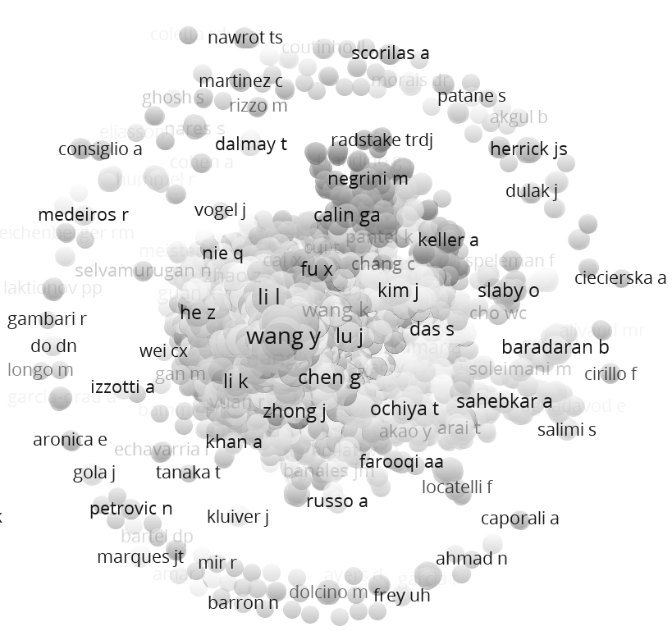
\includegraphics[width=.5\textwidth]{ART_Kawalec/Kawalec-img003bw.png} \\
%	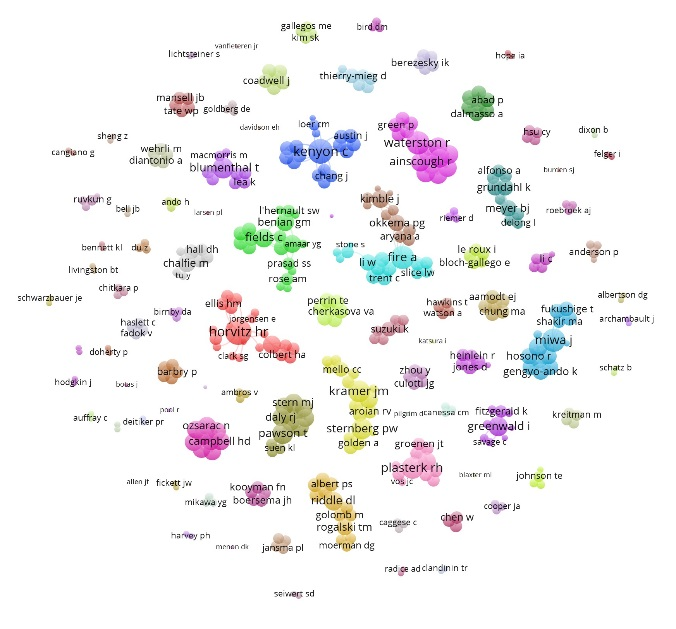
\includegraphics[width=.5\textwidth]{ART_Kawalec/Kawalec-img002.jpg}  &
% 	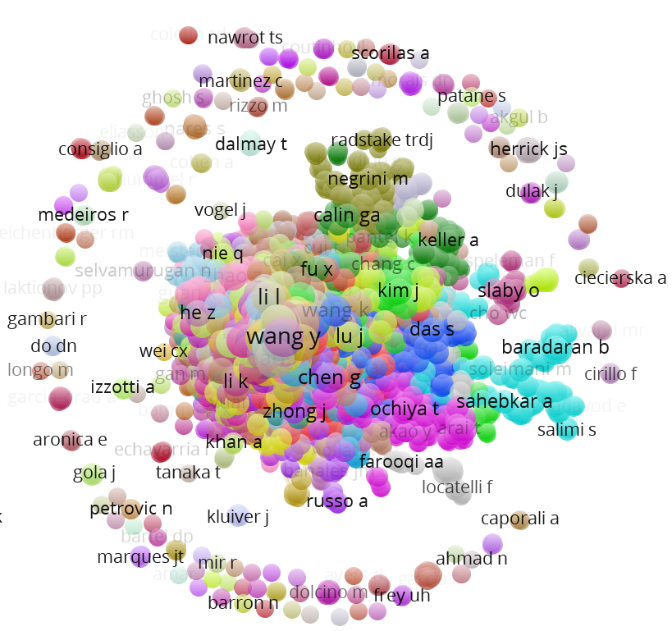
\includegraphics[width=.5\textwidth]{ART_Kawalec/Kawalec-img003.png} \\
\multicolumn{2}{c}{{\centering\bfseries giant component}
}\\
\centering 6\% (of 436 authors) &
\centering\arraybackslash 70\% (of 38 703 authors)\\
\end{tabular}
\end{flushleft}
\caption{Dynamics of microRNA routine – the expansion of size and the giant component of collaborating authors. Source: own analysis of MEDLINE dataset for “microRNAs” as keyword.}\label{fig2kawalec}
\end{figure}

It should be noted, however, that the dynamics between 1993 and 2018 is a very complex and multidimensional process. It cannot simply be captured, as claimed by proponents of particularism, by highlighting some important publications or dates, for it is a continuous process resulting from a set of interacting mechanisms. The discussion of \textit{lin-4} and \textit{let-7} in the remainder of this section illustrates just one aspect of this complexity.

The first microRNAs discovered in \textit{C. elegans lin}-4 and \textit{let}-7 were initially named ``small temporal'' (stRNAs) to emphasize the fact that they are developmentally regulated as well as they control developmental programs
%\label{ref:RNDxU5z6vTHLm}(Lagos-Quintana et al., 2002),
\parencite[][]{lagos-quintana_identification_2002}, %
 such as Dauer larva or vulva formation: ``\textit{lin}-4 and \textit{let}-7 control the timing of postembryonic events by translational repression of target genes, permitting progression from early to late developmental programs'' 
%\label{ref:RNDjC15tfAZXc}(Sempere et al., 2003, p.9).
\parencite[][p.9]{sempere_temporal_2003}. %
 While \textit{let-7} was early identified in a wide class of organisms, \textit{lin-4} was thought to be specific to worms. Early search for new microRNAs in mouse tissue led in 2002 to discovery of \textit{lin-4} ortholog miR-125 which is more widely present in other species, including humans 
%\label{ref:RNDtegoozSxYu}(Yin et al., 2015).
\parencite[][]{yin_progress_2015}. %


Apparently, another important difference between \textit{lin-4} and \textit{let-7} that was noted early on was the recognition of the role of \textit{let-7} in oncogenesis and tumor suppression. Hence, \textit{let-7} has become an object of intense studies as it ``was considered as the most important miRNA for the cancer incidence and progression''
%\label{ref:RNDLaW8XsZykT}(Wang, Jiang and Xu, 2018).
\parencite[][]{wang_comprehensive_2018}. %
 The role of homologs of \textit{lin-4} in oncogenesis was noted later and was less apparent 
%\label{ref:RNDymkacnfBGk}(Sonoki et al., 2005).
\parencite[][]{sonoki_insertion_2005}. %
 The differences between \textit{lin-4} and \textit{let-7}, at least partly, explain the difference in their respective research dynamics as presented in figure \ref{fig3kawalec} which depicts the dynamics of topical expansion of both research lines against the annual growth of the number of publications.
\begin{figure}[h!]
	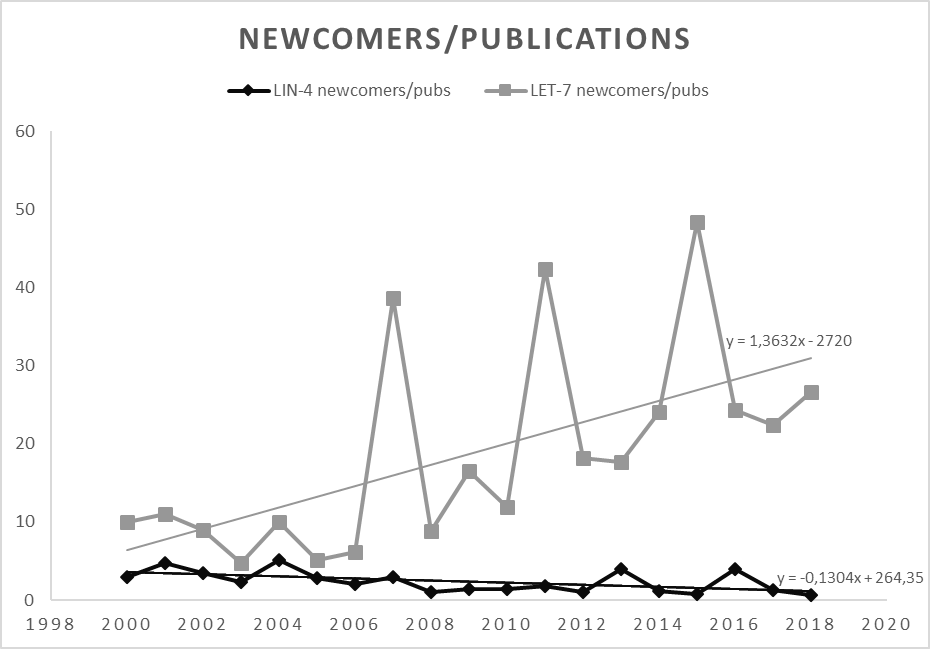
\includegraphics[width=1\textwidth]{ART_Kawalec/Kawalec-img004bw.png}
%	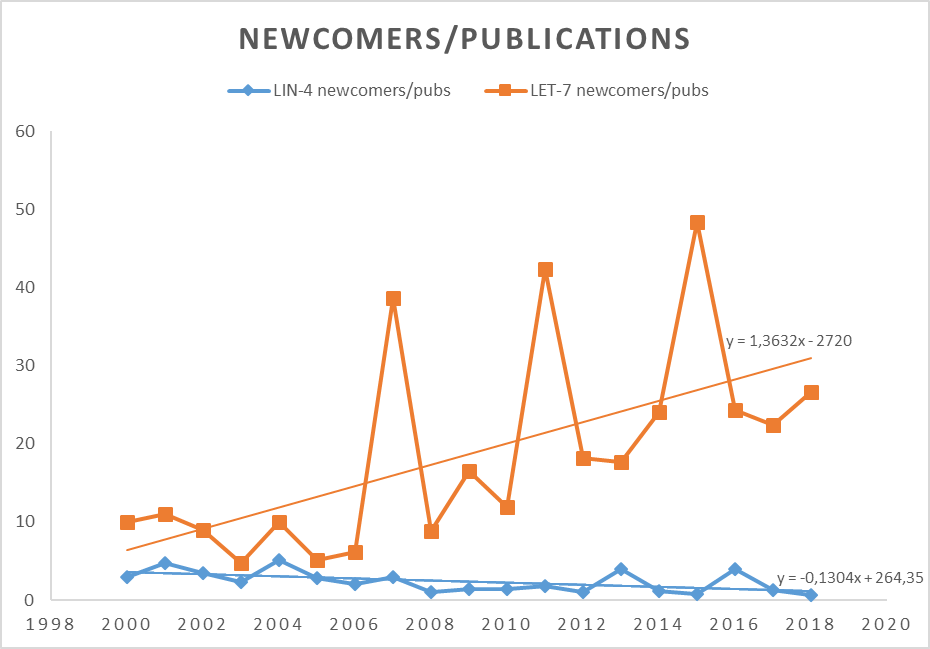
\includegraphics[width=1\textwidth]{ART_Kawalec/Kawalec-img004.png}
	\caption{Newcomer dynamics of MeSH keywords relative to the annual number of publications for the first two microRNAs: \textit{lin-4} and \textit{let-7}. Source: own analysis of MEDLINE datasets for ``\textit{lin-4}'' and ``\textit{let-7}'' as keywords, respectively. The number of hitherto unrecorded MeSH keywords (``newcomers'') for a given year was measured against the annual publication record for ``\textit{lin-4}'' and ``\textit{let-7}'', respectively. The trendlines were estimated as linear functions.}\label{fig3kawalec}
\end{figure}

Interestingly, both processes are characterized by peaks with \textit{let-7} displaying their stronger impact. Those peaks represent a sudden growth of interest in microRNAs and outbursts of hitherto unused MeSH keywords.\footnote{The MEDLINE classificatory scheme of MeSH keywords, in contrast to author keywords, provides a consistent measure of topical expansion of a given research area.} Elsewhere
%\label{ref:RNDMyMMlnwtOG}(Kawalec, 2020)
\parencite[][]{giovagnoli_cognitive_2020} %
 I provided an explanation of this phenomenon in terms of the underlying inherent mechanisms and unexpected external shocks. The account presented here, thus, is a modified processualism as it accommodates unexpected impulses independently from the inherent dynamics of a series of research processes, which are informed by the outcomes of the antecedent ones and, as claimed by D.J. de Solla Price, typically instantiate the logistic curve. The external shocks may be difficult to satisfactorily characterize as they presumably embrace a wide class of phenomena from new discoveries pertaining to microRNAs, through new research methods and instruments to new institutional arrangements, such as installment of new laboratories or funding schemes.

Nevertheless, in the presented case of \textit{let-7} some clues seem quite plausible. The initial discovery of the molecular regulatory mechanism of \textit{let-7} and its high evolutionary conservation
%\label{ref:RNDXszYukj7pQ}(Nelson and Ambros, 2019)
\parencite[][]{nelson_trans-splicing_2019} %
 drew attention of several important research laboratories, such as Bartel's or Tuschl's and resulted in 2001 in a first wave of new microRNAs discoveries, both in \textit{C. elegans} and other organisms. The whole area of microRNAs research was strongly impacted by introduction around 2006 of new instruments of ``next-generation sequencing'' enabling high-throughput analysis. This was reflected in a subsequent proliferation of topics that peaked in 2007, including identification of \textit{let-7} targets, such as the gene \textit{Hmga2} (\textit{High Mobility Group A2}) having being already well-known for its expression ``in a wide variety of benign and malignant tumors'' 
%\label{ref:RNDHB1OgkqYEs}(Mayr, Hemann and Bartel, 2007, p.1576).
\parencite[][p.1576]{mayr_disrupting_2007}. %
 Demonstrating thus the high diagnostic and therapeutic potential of \textit{let-7} 
%\label{ref:RNDqoFLg9dZgk}(Johnson et al., 2007; Kuehbacher et al., 2007; Park et al., 2007; Cinkornpumin et al., 2017; Pobezinsky and Wells, 2018; Roos et al., 2018).
\parencites[][]{johnson_let-7_2007}[][]{kuehbacher_role_2007}[][]{park_let-7_2007}[][]{cinkornpumin_small_2017}[][]{pobezinsky_lets_2018}[][]{roos_pharmacologic_2018}. %
 Later, the role of \textit{let-7} was recognized in post-transcriptional control of innate immune responses to pathogenic agents and allergic inflammation linking this microRNA to adaptive immunity 
%\label{ref:RNDUAP1ignAmN}(Schulte et al., 2011; Kumar et al., 2011).
\parencites[][]{schulte_analysis_2011}[][]{kumar_let-7_2011}. %
 Finally, the year 2015 marks an intense exploitation of the therapeutic and diagnostic potential of the circulating microRNAs that are present in bodily fluids and therefore have good potential as an accessible and attractive biomarker.

\section{Concluding remarks}
As demonstrated in figure \ref{fig3kawalec}, although the interest in \textit{lin-4} is slightly declining, like \textit{let-7} it still remains an object of a steady line of research that brings about new insights. The mechanism of developmental timing pathway of \textit{lin-4} and \textit{let-7} as the first ``small temporal'' or ``heterochronic'' regulatory genes appears to be quite universal
%\label{ref:RND1PazrnVE9B}(Bracht et al., 2010).
\parencite[][]{bracht_regulation_2010}. %
 On the other hand, however, \textit{let-7} is apparently more prone to external shocks. It, at least partly, derives from its high therapeutic and diagnostic potential. Thus, we have a clear illustration of both general problems of particularism discussed in the previous section. An attempt to pin down the milestones in the development of research on \textit{let-7} may be quite misled by the external shocks that strongly affect the tangible dynamics of this line of research.

Consider now the reference class problem. The often made claim that Ambros and his collaborators discovered microRNA in 1993 is obviously a short-cut. To appreciate the general nature of the non-coding mechanism of \textit{lin-4} the discovery of \textit{let-7} was needed. Moreover, several other discoveries were needed to reveal microRNAs's biogenesis, their targets, different forms in different organisms, role in developmental and pathogenic processes, etc. Hence, if---following the particularist practice---we would single out the 1993 paper by Ambros and collaborators as the source of the breakthrough this will leave us with a very simplistic notion of ``microRNA''. Similarly, an alternative way to pin down the discovery with regard to the combination of the two 1993 papers by Ambros's and Ruvkun's teams and the latter's two 2000 papers would face similar problems. On the other hand, focusing on---all, or one, of---the most spectacular peaks in the dynamics of \textit{let-7} may misguide the real cognitive mechanism and turn us, instead, to the external shocks.

Particularist atttempts to pin down the moment of discovery, or its most important outcome, may have an important social role, such as prestigious awards, policy decision-making or public communication of science. Nevertheless, the integrative explanation of the dynamics would need to acknowledge the complexity of the whole process of discovery.

\section{Acknowledgments }
An earlier version of this paper was presented on January 21 in 2019 at the PAU Commission on the Philosophy of Science. I appreciate the comments received during the discussion that helped me to improve the final draft.

I am grateful to the anonymous Reviewers for their constructive comments and insightful recommendations which helped to improve the quality of the paper.

\end{artengenv}